\section{Design}
The system will be a frontend for a user to interact with the SpaceTraders API through a console prompt and graphical interface. And is described by the structure chart below:


\shadowbox{
    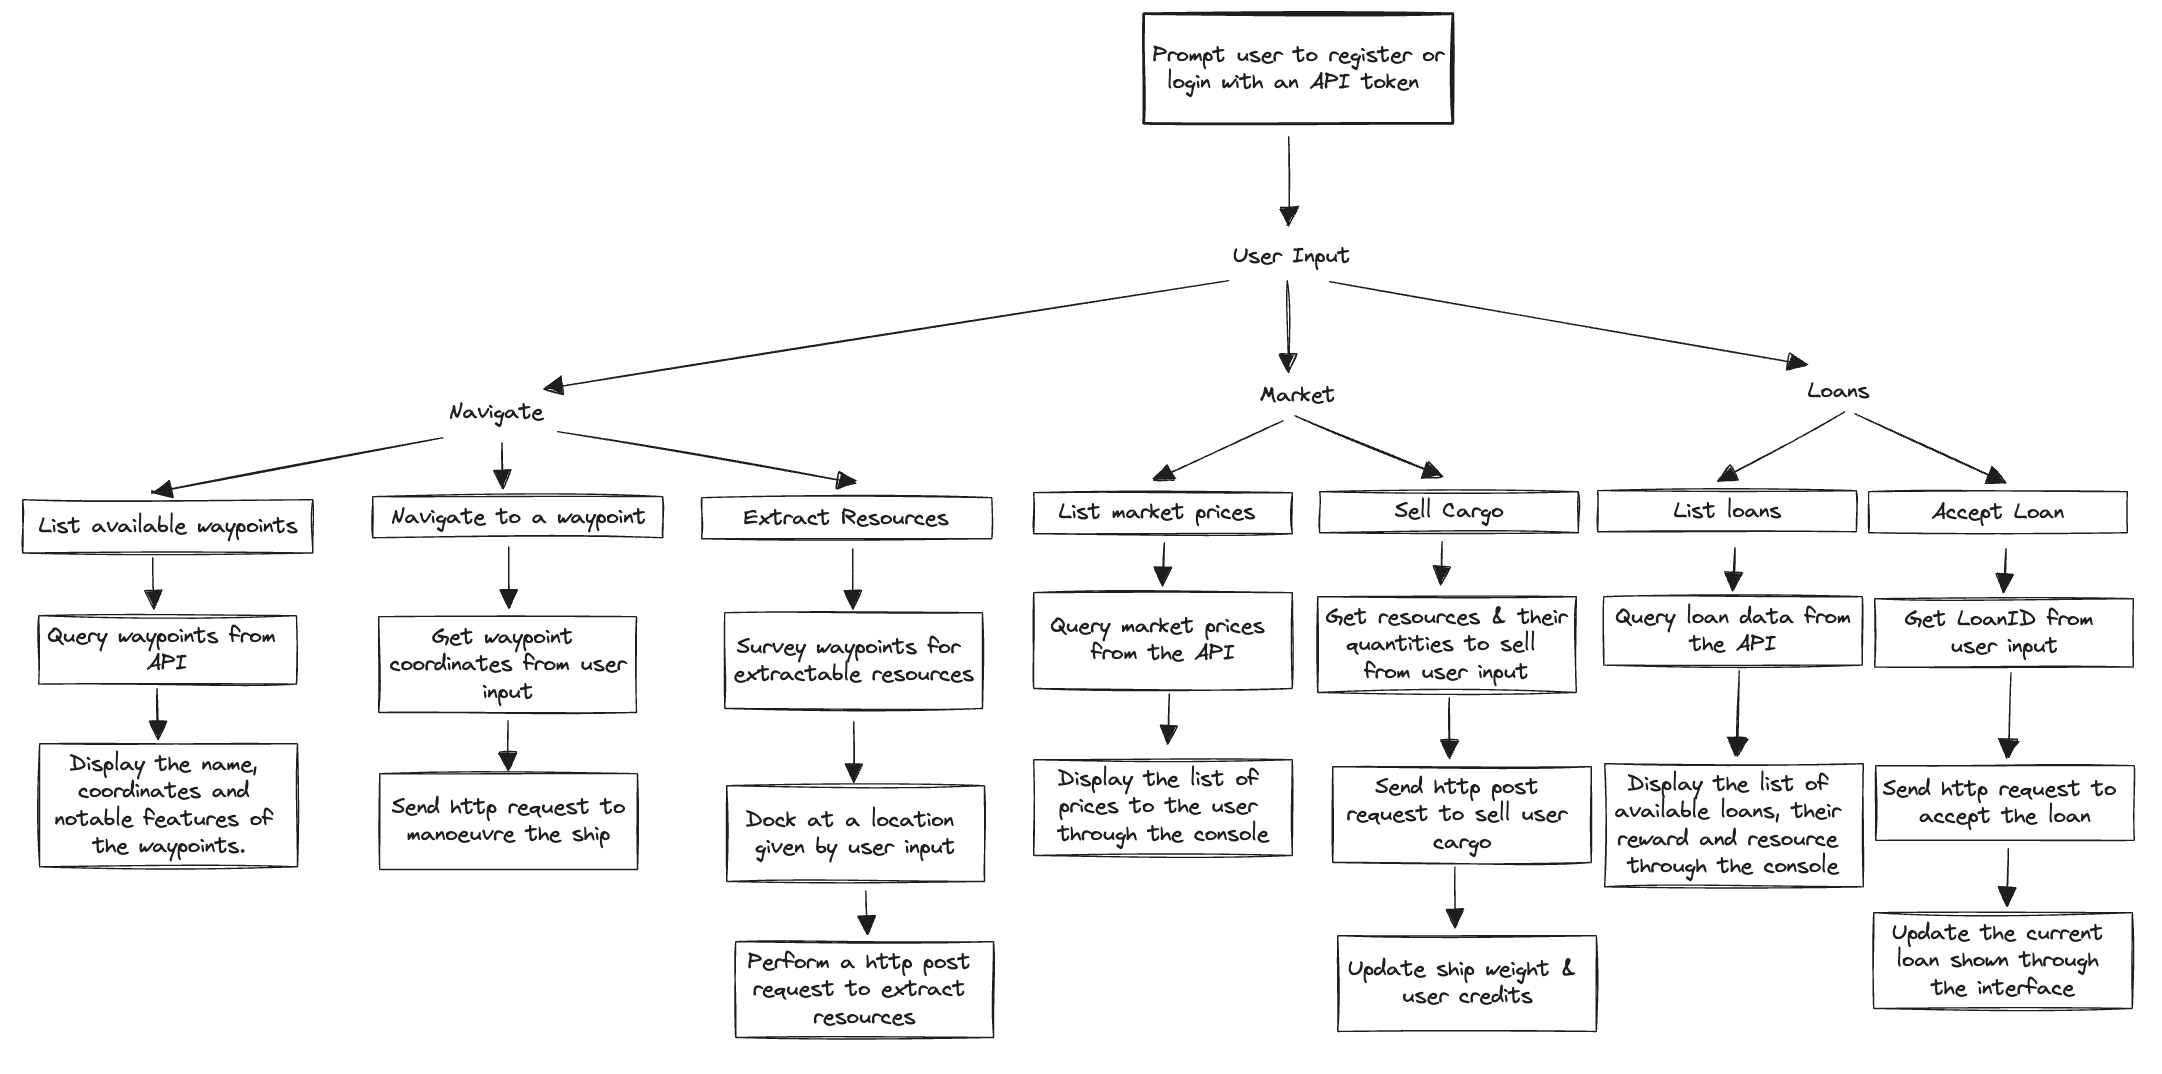
\includegraphics[angle=90, origin=c, width=11cm]{system-diagram.png}
}

\subsection{Data Design}
Data entering the system will be queried from the SpaceTraders API, and the JSON responses from http requests will have to be parsed into a series of structs which can be passed as parameters to maintain state. A \texttt{GameState} class will hold references to the other classes required for API calls, or communicating information to the user and will be defined as below. The waypoints vector will be used for displaying a graphical star map on the right of the screen, and the Agent reference, for storing the symbolic name and token key for future API requests.
\begin{lstlisting}
struct GameState {
    agent: &Agent,
    waypoints: Vec<Waypoint>,
}
\end{lstlisting}

The Agent class will store all account information that may be displayed through the interface or required for API calls, including: the agent's symbolic name, API token, current loan, and credits. It also contains a vector of Ships composing the fleet, thus mitigating the need for querying the API every time information is requested – and the structs only have to be rebuilt when performing modifying requests – thus reducing latency by minimising requests.
\begin{lstlisting}
struct Agent {
    token: &str, 
    symbol: &str,
    credits: u32,
    curr_loan: &Loan,
    fleet: Vec<Ship>,
} 
\end{lstlisting}

The Agent class contains references to both the \texttt{Ship}, and \texttt{Loan} classes defined by the specification below. Both will be created to parse the json response of a request into an organised structure, and stored to later be queried when users request information on their fleet or loans.
\begin{lstlisting}
enum FlightMode {
    CRUISE,
    BURN,
    DRIFT,
    STEALTH,
}

struct Ship {
    flight_mode: FlightMode,
    curr_waypoint: &Waypoint,
    fuel: i32,
    curr_weight: u32,
    max_weight: u32,
}

enum Resource {
    IRON_ORE,
    COPPER_ORE,
}

struct Loan { 
    reward: i32,
    resource: Resource,
    expiration_date: DateTime,
}
\end{lstlisting}

A similar interface definition of the \texttt{Waypoint} struct can be created. Instances of these will be stored in a vector attribute of the \texttt{GameState} struct, and used to visually display a map of the star system, as well as to be referenced by ships to indicate their current position.
\begin{lstlisting}
enum Trait {
    SHIPYARD,
    MARKET,
    ASTEROID
}

struct Waypoint {
    symbol: &str,
    coordinate: [i64; 2],
    trails: Vec<Trait>,
}
\end{lstlisting}
These data structures will store the parsed JSON from the SpaceTraders requests, and will be passed around as state through references from the \texttt{GameState} struct which will display the required data contained within these structs to the user. 

\subsection{Screen Layouts}
The Terminal User Interface (TUI) will be split into 4 main components, the header – containing the application title, agent symbol, and current loan; the console - containing a history of previous commands and their textual output; a prompt - where the user will enter commands; and the graphical display - where information regarding the SpaceTraders star system such as waypoints and ship locations can be communicated.

\shadowbox{
    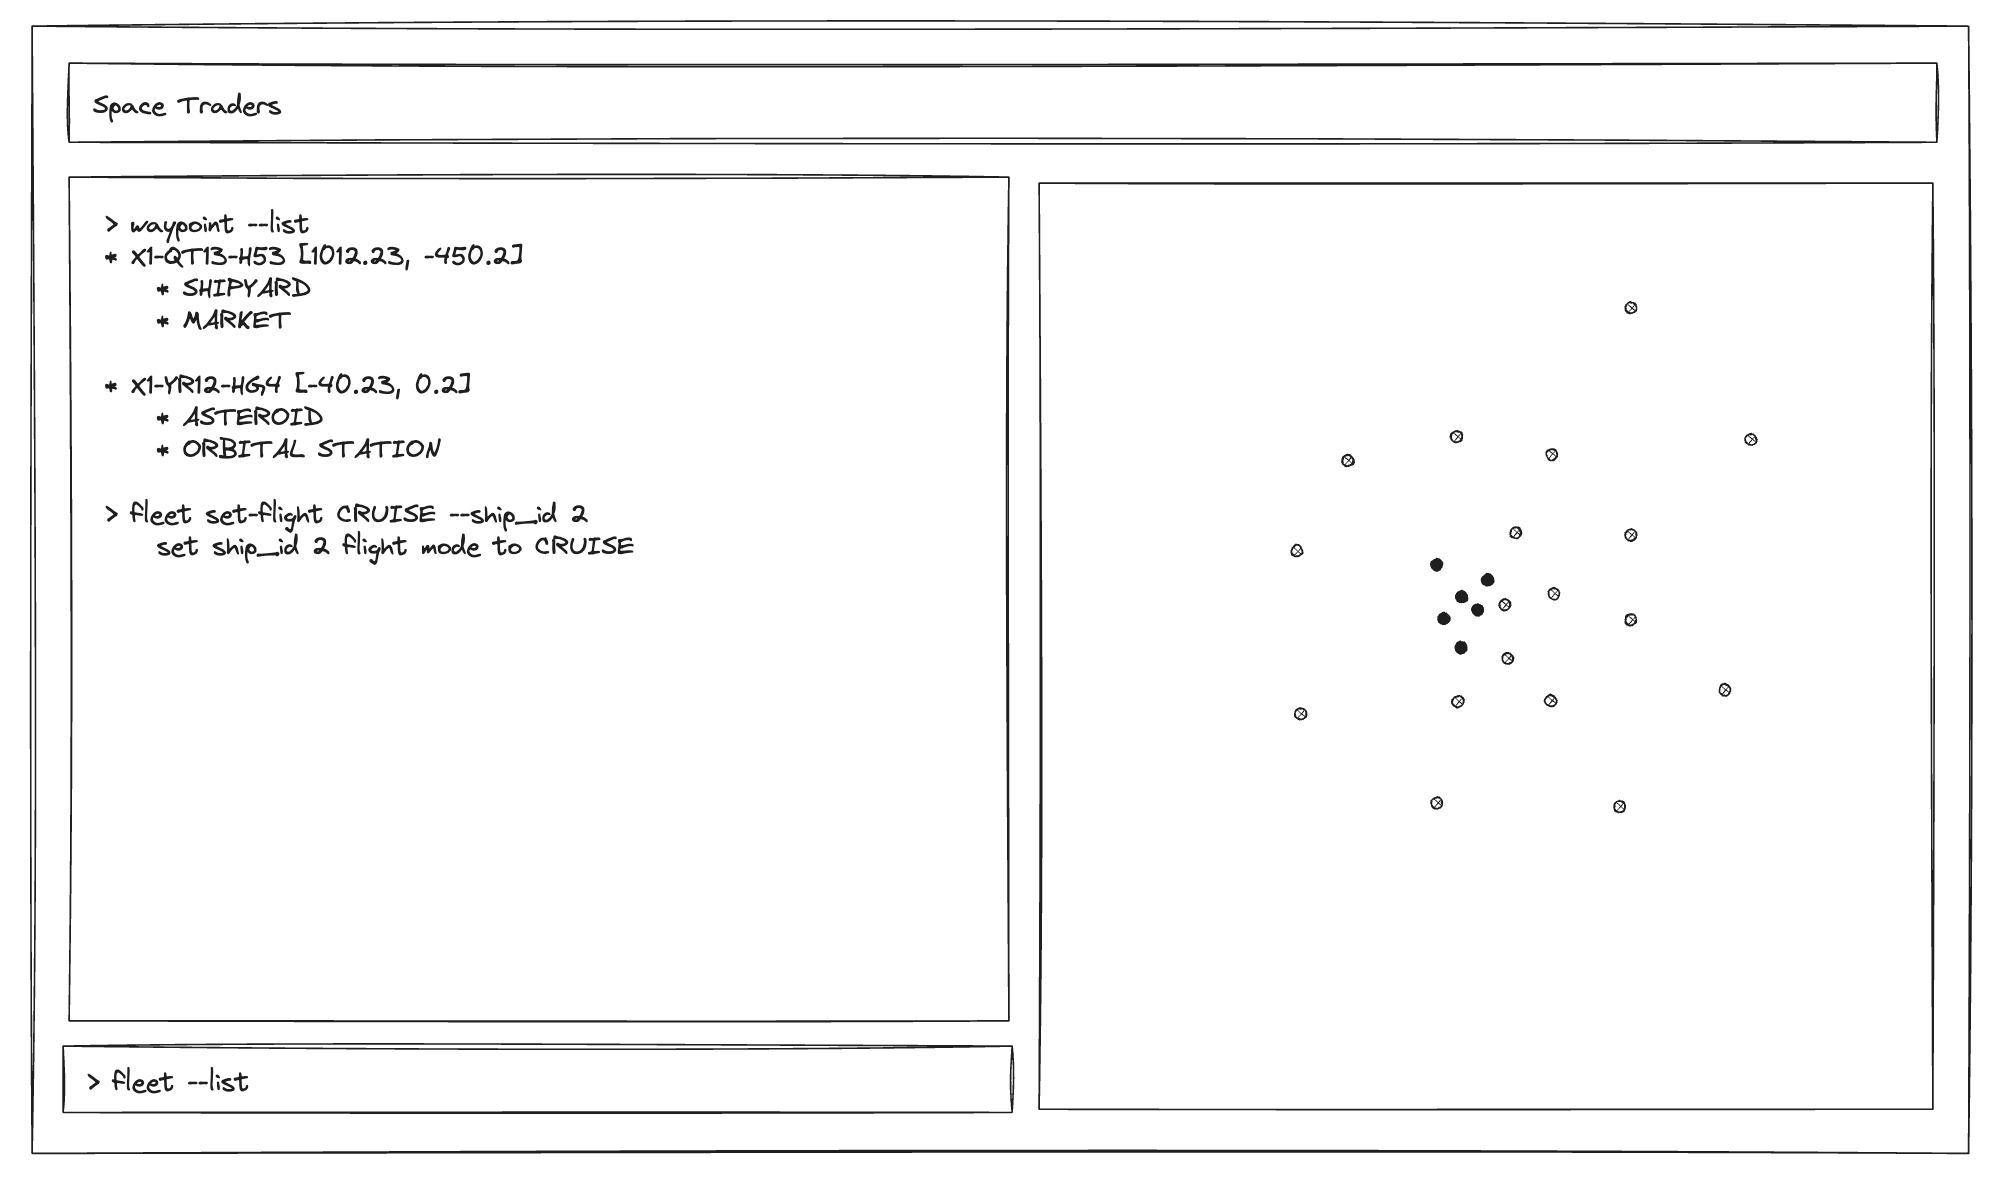
\includegraphics[width=11cm]{frontend-mockup.png}
}

\subsection{Key Algorithms}
\subsubsection{Managing \& Purchasing a Ship}
The first algorithm will handle the process of purchasing a ship - and consist of locating nearby shipyards, listing the ships contained within a particular shipyard given by its waypoint symbol, and purchasing the desired ship from said shipyard. The algorithm can be decomposed into the following tasks:

\bigskip

\shadowbox{
    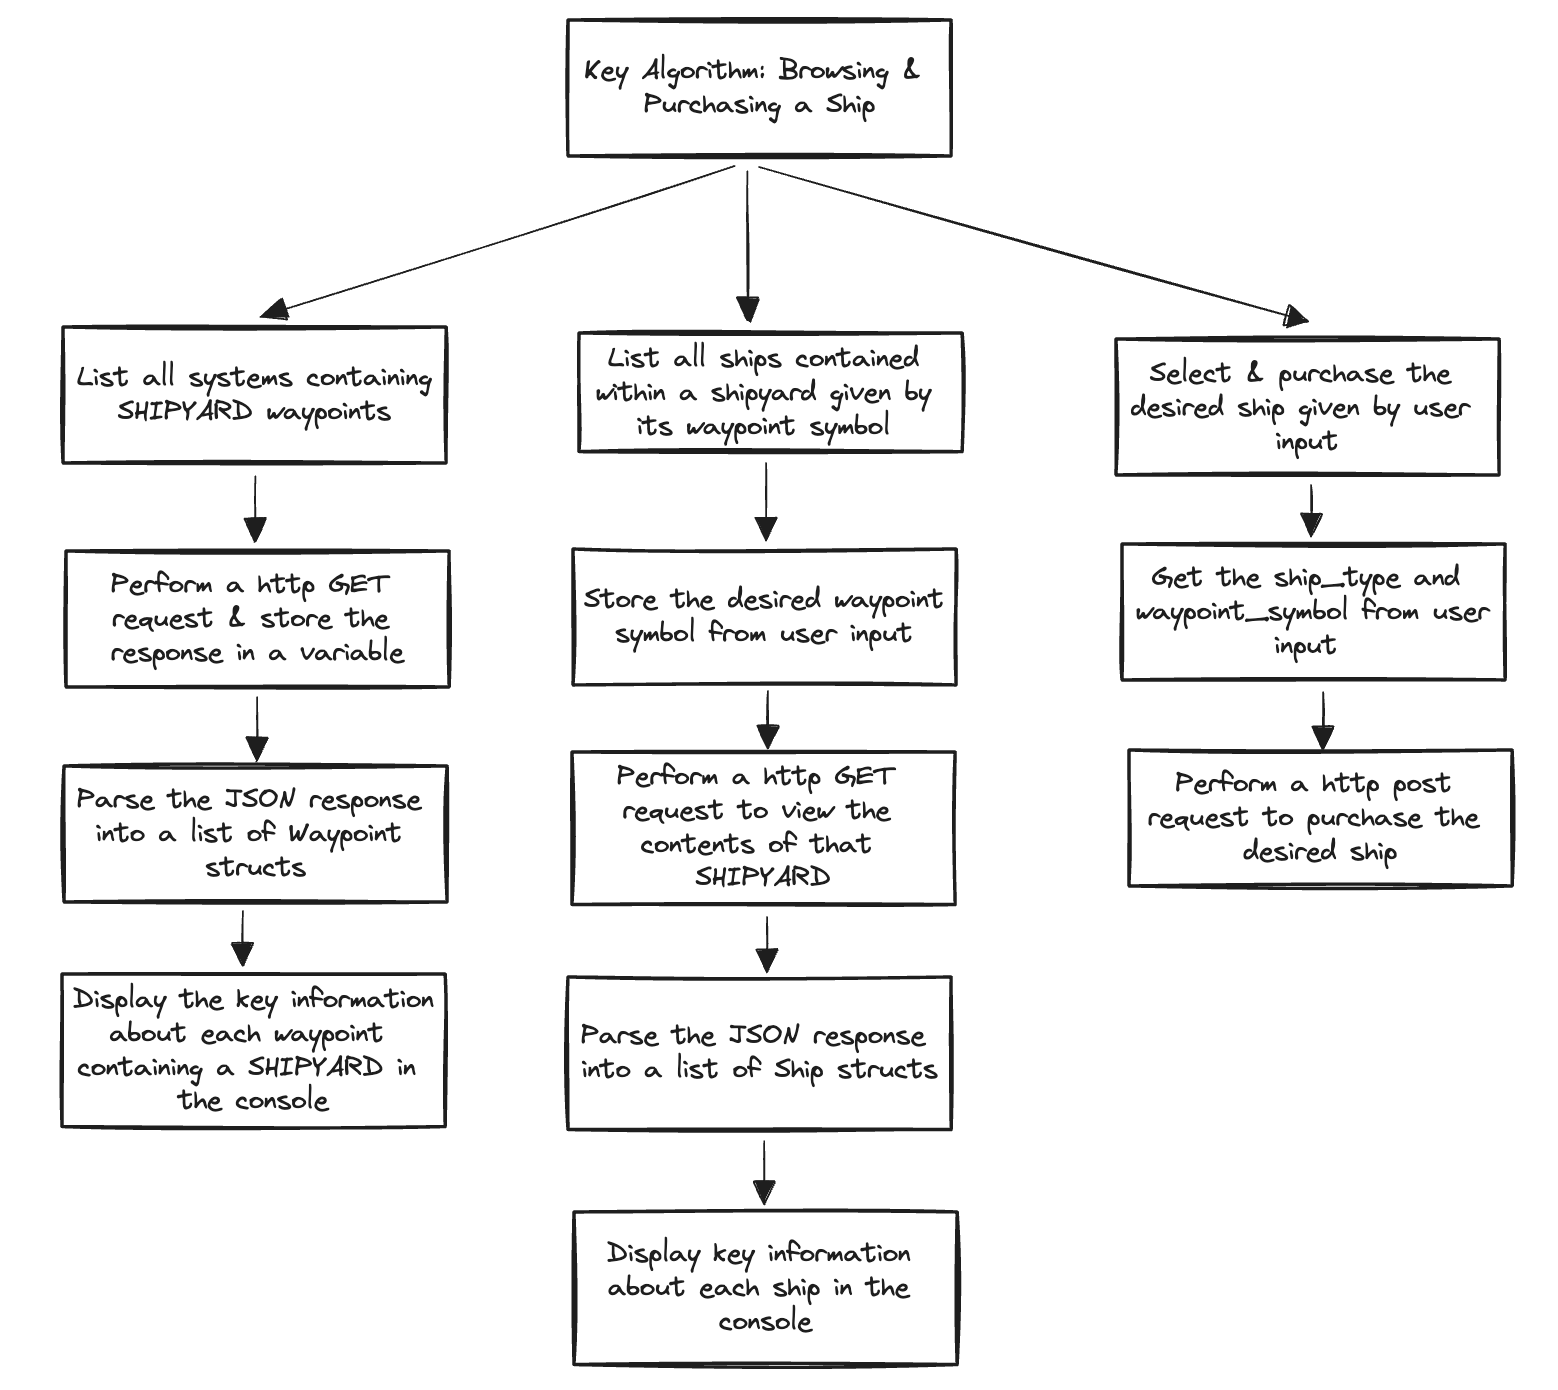
\includegraphics[width=11cm]{algorithm.png}
}

\subsubsection{Listing Waypoints containing a Shipyard}
The first part of the algorithm consists of performing a parameterised get request, setting \texttt{shipyard} as a trait required for the JSON of such a waypoint to be returned. The algorithm will then parse this data into a structure, and print it to the console. The format wil be the waypoint's type, symbol, coordinates and then a list of traits e.g. (SHIPYARD, VOLCANIC, etc..). The following pseudocode will represent this algorithm:
\begin{lstlisting}[language=C]
PROCEDURE ListWaypointsWithTrait(STRING trait)
    response <- GET https:/api.spacetraders.io/v2/systems/X1-ZB92/waypoints?traits={trait}

    FOR waypointJSON IN response DO 
        waypoint = Waypoint::FROM(waypointJSON)

        OUTPUT "{waypoint.symbol} - {waypoint.type}, ({waypoint.x}, {waypoint.y}):" 
        FOR trait in waypoint.traits DO
            OUTPUT "*{trait.symbol}\n"
        END
    END
ENDPROCEDURE
\end{lstlisting}
\subsubsection{Listing the contents of a Shipyard}
The second part of the algorithm will list the contents of a particular shipyard (given by user input), and will involve the same process of parsing the JSON repsonse into a series of structs, with which an easy to digest decomposition of all the ships and their features can be displayed through the console.
\begin{lstlisting}
FUNCTION ListShipyardContents() RETURNS Ship[]
    waypoint <- INPUT "Enter a waypoint symbol:"
    response <- GET https://api.spacetraders.io/v2/systems/X1-ZB92/waypoints/{waypoint}/shipyard'

    Ships <- []
    FOR shipJSON in response["ships"] DO 
        ship <- Ship::FROM(shipJSON)
        OUTPUT """
        {ship.type} {ship.name} {ship.price}
        {ship.description}
        """
        Ships.push(ship)
    END

    RETURN Ships
ENDFUNCTION
\end{lstlisting}
\subsubsection{Purchasing a ship from a Shipyard}
Finally, after the the contents of a particular shipyard has been listed and the user has made a decision on which to purchase, they will be prompted for the type of the ship they wish to purchase. Then before the post request is made, the user's credits will be checked against the price of the ship - and a suitable message will be output if they do not have the funds. Else, a http post request will be sent to the SpaceTraders API to purchase the ship. 
\begin{lstlisting}
PROCEDURE PurchaseShip(GameState)
    ShipType <- INPUT "Enter the ship you wish to purchase:"
    IF GameState.agent.credits < ships["ship_type"].price
        OUTPUT "You do not have sufficient funds to purchase this ship"
    ELSE 
        POST --url 'https://api.spacetraders.io/v2/my/ships'
        --header 'Content-Type: application/json'
        --data '{
           "shipType": "{ShipType}",
           "waypointSymbol": "{Waypoint}"
          }'
    ENDIF
ENDPROCEDURE
\end{lstlisting}